\part*{第2章\\人間のチーム行動解析}
\chapter{人間のチーム行動解析}
%章番号が不要な場合は『\chapter*{概要}』とする
% =============================================
% セクション開始
%
% =============================================
\section{緒言}
本章では,人間のチーム行動の解析及びロボットへの適応について議論するため,ニューラルネットワークに代表される学習機能を有するアルゴリズムを取り上げる.ニューラルネットワークの特徴として,様々なシステムに対して寛容であり,学習を行うことで非線形的な信号に対しても適応可能であるようなロバスト性を有する.

% =============================================
% セクション開始
%
% =============================================
\clearpage
\section{階層型ニューラルネットワーク(MLP)}
階層型ニューラルネットワークは,入出力間の写像関係を学習して構築され,信号が常に入力層から出力層方向に向かう脳型情報処理アルゴリズムである.入力データと出力目標データの対からなる訓練データを多数組与え,ネットワークがこれらの入出力関係を再現するよう結合荷重を修正していくことで学習が進む.

% =============================================
% セクション開始
%
% =============================================
\clearpage
\section{自己組織化マップ(SOM)}
自己組織化とは,局所的な相互作用から地域的に順序づけられた構造が導かれることであり,複数の要素から構成されるシステムが他からの制御を得ることなく,時間とともに何らかの意味で自発的に秩序化する過程である.神経回路の構造は,脳内においてこの自己組織化の代表的な例として挙げられる.1956年にSperryによってはじめられた視覚神経通路の発達における位相的順序を保持した状態での網膜位相マップの構築を目的としたモデル化が,自己組織化の位相形成原理についてのモデル化の先駆けとなり,Von der Malsburg\cite{von_der_Malsburg}が特徴選択における皮質細胞の局所的な順序づけを目的としたシナプス学習を含む自己組織化過程を導入するなど,創刊がある神経活動によって駆動される位相的なマップの形成に関係した自己組織化の要素が神経活動による位相マップの初期の形成には存在するという結論が主流となった.その後,1976年にWillshaw とvon der Malsburg\cite{WILLSHAW}によって,本質的には同様の幾何学的関係がある離散的な格子間での類似関係を検出する自己組織化処理モデルが,自己組織化マップ(Self-Organizing Map : SOM)として提案され,SOMは,教師なし学習であり,生命の神経回路による情報処理に近い競合学習として知られるようになった.\\
Kohonen は前述したモデルからさらに,類似関係があるものではない,かつ幾何学条性格である必要もない離散的格子上に連続した入力君間からマップ化することを目的として学習アルゴリズムを変更した\cite{The_Eye_and_the_Brain}.より強度な自己組織化効果を得るために,近傍関係を学習に導入するため荷重更新規則を修正し,これらの近傍関係によって広がった範囲が時間経過にともない縮まる要素も追加した.これにより,SOMのアルゴリズムとして,Kohonenモデルが一般的となり,本論文中にあいてもKohonenモデルを取り扱う.\\
この構造により,多次元入力ベクトルの低次元化が出力そうにて可能であり,特徴が近似している入力ベクトルほど,近くに配置される.SOMの応用例としては,複雑なデータの二次元表示への可視化があり,クラスタリング技術と同様に,抽象化の創造が可能である.優れた補間性能を保つために,学習データの一般化が可能であり,未知な入力データに対しても妥当性の高い出力が期待される.
\subsection{競合学習}
競合学習は階層型ニューラルネットワークにおいて重要な懸念である.同一の入力に対し,各々のニューロンが活性度を競い合う側方相互作用が利用される.具体的に競合学習としてのSOMは,入力層と出力層からなり,入力層(入力空間V)の各入力サンプル(入力ベクトルv(t))は全ての出力層ニューロンと結合し,結合には結合荷重$w_i$が付加されている.ここでtは時間座標であり,N個の出力層ニューロンは,$i=1,2,・・・,N$とラベル付けされている.(Fig\ref{fig:SOM_Algorithm})そして,近くのニューロンとの結合は興奮性(正の結合荷重)があり,より遠方のニューロンとの結合には抑制性(負の結合荷重)がある状態で出力層のニューロンは活性化するために競合する.

\clearpage %-------------------------図-----------------------------------------

\begin{figure}[ht]
  \begin{center}
  
    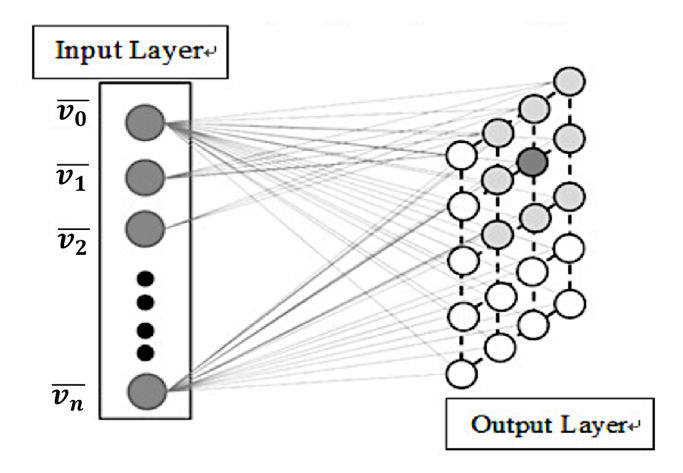
\includegraphics[clip,width=15.0cm]{figure/02_01_Overview_of_SOM_algorithm.eps}
    \caption{Observation of SOM algorithm}
    \label{fig:SOM_Algorithm}
    
  \end{center}
\end{figure}

\clearpage%-------------------------図-----------------------------------------


\subsection{アルゴリズム}
KohonenのSOMアルゴリズム\cite{Kohonen}は,大きく競合段階と協調段階の二つの改装で構成される.最初の段階ではまず,入力に対して,最整合ニューロン(Best Matching Unit : BMU)の選択すなわち勝者を選択する.次に,その最整合ニューロンおよびその直近の格子の荷重変更が行われる.以下に,これら二つの段階について述べるが,本研究では,新しい入力ベクトルの投入のたびに,荷重更新を行う増分学習(オンライン学習)ではなく,全入力ベクトルの協業段階が行われた後に,生成できる全入力が考慮された荷重更を行う,バッチ型SOM[?]を用いる.これにより,入力ベクトルの投入順番による出力への影響を考慮する必要がなくなる.よって,以降は本研究で用いたバッチ型SOMについて述べているため,バッチ型SOMへの変更に伴い,入力空間$V$を$ \mu = 1, \cdots,M$の$M$個のサンプルからなる固定の学習ベクトル集合$\{v^\mu\}$として定義する.
\subsubsection{競合段階}
競合段階では,各入力ベクトル$v^\mu$に対する最整合ニューロンについて式(\ref{1})を用いて選択する.BMUの決定方法としては,内積距離規則やユークリッド距離規則が考えられる.内積距離規則は生物学的モデルに類似しているため,多くその方面で用いられているが,今回は生物学的なモデルとしてSOMを扱う必要がないため,ユークリッド距離規則によるBMU決定を採用する.ユークリッド距離を用いる場合,結合荷重改め,ベクトル量子化の観点から参照ベクトルと呼ぶこととする.ここでは,勝者$j*$とラベル付けする.また,$\|.\|$はユークリッド距離を表している.
\begin{equation}
\label{1}
  i^* = argmin||w_i - v^\mu||
\end{equation}

\subsubsection{協調段階}
協調段階では,ニューロンが発火(BMUが決定されること)することにより,その周囲のニューロンも協調的に発火しやすくなるように荷重更新に影響を与える段階である.各丹生論の参照ベクトル$w_i$を式(\ref{2})により更新する.ここで,$t$は学習回数を示す変数であり,総学習回数を$t_{max}$とする.$\eta$は学習係数である.

\begin{equation}
\label{2}
w_i(t+1) = w_i(t)+\frac{\eta}{M}・\Delta w_i
\end{equation}

ただし,参照ベクトルの増減値$\Delta w_i$は,次式(\ref{3})で示される.

\begin{equation}
\label{3}
\Delta w_i(t +1) = \Delta w_i(t)+\Lambda(i,i^*,\sigma_\Lambda)・(v^\mu-w_i)
\end{equation}

ここで,$\Lambda$はニューロン$i$と $i^*$の格子座標$r$と$r^*$での尺度調整を行う近傍関数である.勝者の位置に関して左右対称であり,勝者からの格子距離が増加するにしたがって単調に減少する関数でなければならない.今回は,もっとも一般的なガウス型近傍関数(式\ref{4}参照)を用いた.(図\ref{fig:Sigma_3_3D}-\ref{fig:Sigma_1_2D}参照)$\sigma_\Lambda$は,その範囲(標準偏差)である.

\begin{equation}
\label{4}
\Lambda(i, i^*) = \exp(-\frac{{\|r_i-r_{i^*}\|}^2}{{2\sigma_\Lambda}^2})
\end{equation}

先に述べた,近傍関数によって広がった範囲が時間経過にともない縮まる要素として,標準偏差,式(\ref{eq:5})によって学習回数とともに小さな値をとる.(図\ref{fig:Time variation of standard deviation}参照)

\begin{equation}
\label{eq:5}
\sigma_\Lambda={\sigma_{\Lambda_0}}\exp(-2{\sigma_{\Lambda_0}}\frac{t}{t_{max}})
\end{equation}

\begin{figure}[H]% --------------------------図----------------------------------
    \begin{tabular}{cc}
      %---- 最初の図 ---------------------------
      \begin{minipage}[t]{0.45\hsize}
        \centering
        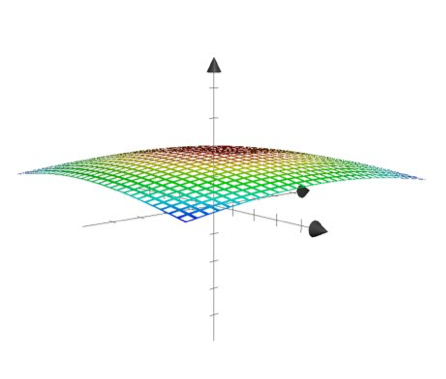
\includegraphics[keepaspectratio, scale=0.8]{Figure/Sigma_3_3D.eps}
        \caption{3D View of $\sigma_\lambda =3 $}
        \label{fig:Sigma_3_3D}
      \end{minipage} &
      %---- 2番目の図 --------------------------
      \begin{minipage}[t]{0.45\hsize}
        \centering
        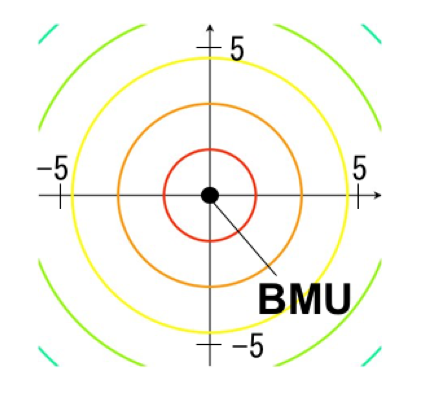
\includegraphics[keepaspectratio, scale=0.8]{Figure/Sigma_3_2D.eps}
        \caption{2D View of $\sigma_\lambda = 3$}
        \label{fig:Sigma_3_2D}
      \end{minipage}\\
      %---- 3番目の図---------------------------
      \begin{minipage}[t]{0.45\hsize}
        \centering
        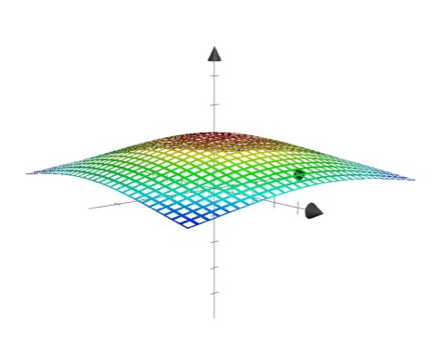
\includegraphics[keepaspectratio, scale=0.8]{Figure/Sigma_2_3D.eps}
        \caption{3D View of $\sigma_\lambda =2 $}
        \label{fig:Sigma_2_3D}
      \end{minipage} &
      %---- 4番目の図 --------------------------
      \begin{minipage}[t]{0.45\hsize}
        \centering
        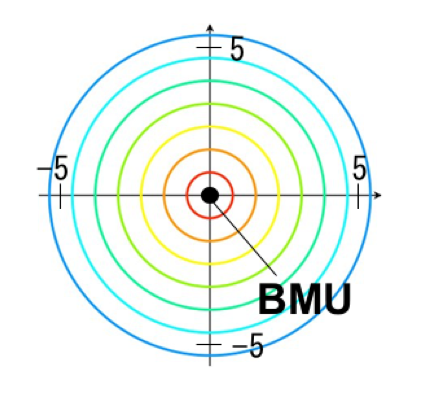
\includegraphics[keepaspectratio, scale=0.8]{Figure/Sigma_2_2D.eps}
        \caption{2D View of $\sigma_\lambda = 2$}
        \label{fig:Sigma_2_2D}
      \end{minipage}\\
      %---- 5番目の図 ----------------------
      \begin{minipage}[t]{0.45\hsize}
        \centering
        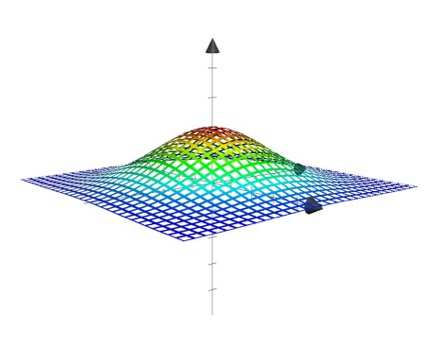
\includegraphics[keepaspectratio, scale=0.8]{Figure/Sigma_1_3D.eps}
        \caption{3D View of $\sigma_\lambda =1 $}
        \label{fig:Sigma_1_3D}
      \end{minipage} &
      %---- 6番目の図 --------------------------
      \begin{minipage}[t]{0.45\hsize}
        \centering
        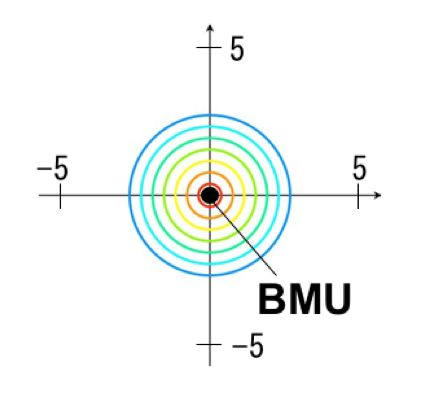
\includegraphics[keepaspectratio, scale=0.8]{Figure/Sigma_1_2D.eps}
        \caption{2D View of $\sigma_\lambda = 1$}
        \label{fig:Sigma_1_2D}
      \end{minipage}\\
      %---- 図はここまで ----------------------


    \end{tabular}
\end{figure}% --------------------------図----------------------------------

\clearpage %-------------------------図-----------------------------------------

\begin{figure}[ht]
  \begin{center}
  
    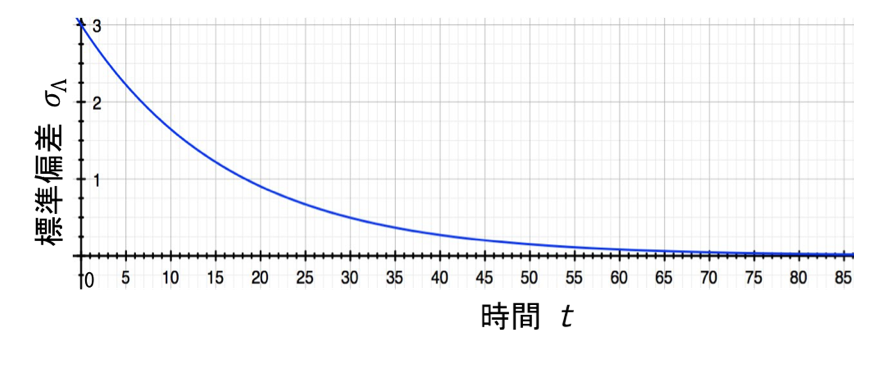
\includegraphics[clip,width=15.0cm]{figure/Time_variation_of_standard_deviation.eps}
    \caption{Time variation of standard deviation}
    \label{fig:Time variation of standard deviation}
    
  \end{center}
\end{figure}

\clearpage%-------------------------図-----------------------------------------

% =============================================
% セクション開始
%
% =============================================
\section{解析実験}
実験は,大きく分けて以下の3つの目的について行う.

\begin{enumerate}
  \item 普段からチーム行動をしているチームとしていないチームで差がでるのか.
  \item 人間によるサッカーにおいて同チームの仲間との位置関係は,SOMのクラスタリングとどう影響するか.
  \item 人間によるサッカー(普段からチームプレーをしているチーム)とロボットによるサッカーの試合では,SOMにできるクラスタの観測はどう異なるか. 
\end{enumerate}

\subsection{観察対象試合}
今回観察対象とする試合は,Table\ref{table1}に示す3試合である.

\begin{table}[htb]
	\begin{center}
	\caption{Observation}
	\begin{tabular}{|c|c|c|}\hline
		\label{table1}
	 	試合名 & プレイヤー & チーム行動  \\ \hline \hline
	 	A & 人間 & 慣れていない  \\
   	 	B & 人間 & 慣れている \\
   		C & ロボット & 慣れている \\ \hline
	\end{tabular}
	\end{center}
\end{table}

試合Aについての観察対象は,Fig\ref{fig:A}に示しており,九州工業大学の大学生の即席チーム同士の試合である.また,試合Bについては,普段から,フットサルチームとして活動されているチーム同士の試合である.(Fig\ref{fig:B}参照)最後に,試合Cは2016年に行われたロボカップ世界大会中型リーグ決勝戦でのオランダチーム(Tech United Eindhoven)と中国チーム(Water)の試合である.(FIg\ref{fig:C}参照)

\clearpage %-------------------------図-----------------------------------------

\begin{figure}[ht]
  \begin{center}
  
    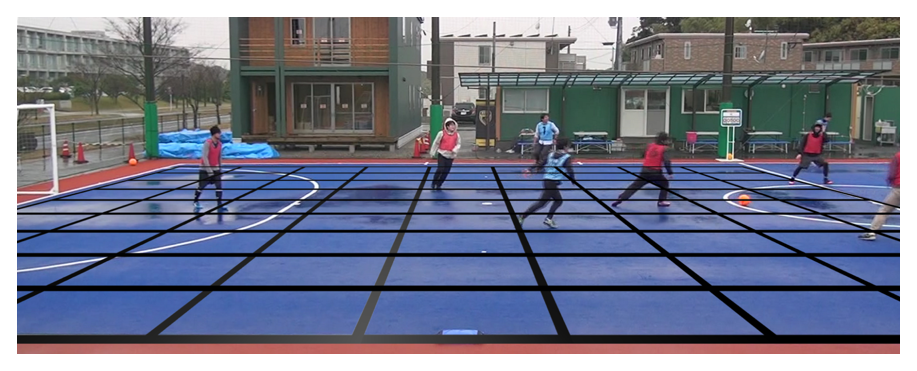
\includegraphics[clip,width=15.0cm]{figure/Observation_target_game_A.eps}
    \caption{Observation target game A}
    \label{fig:A}
    
    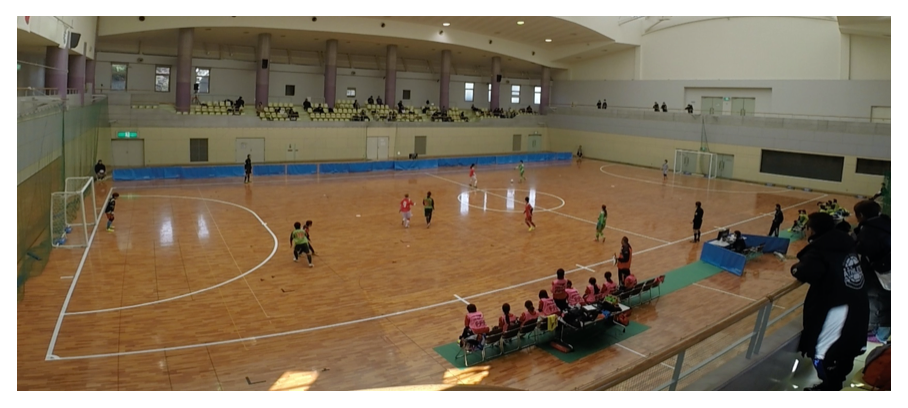
\includegraphics[width=15.0cm]{figure/Observation_target_game_B.eps}
    \caption{Observation target game B}
    \label{fig:B}
    
    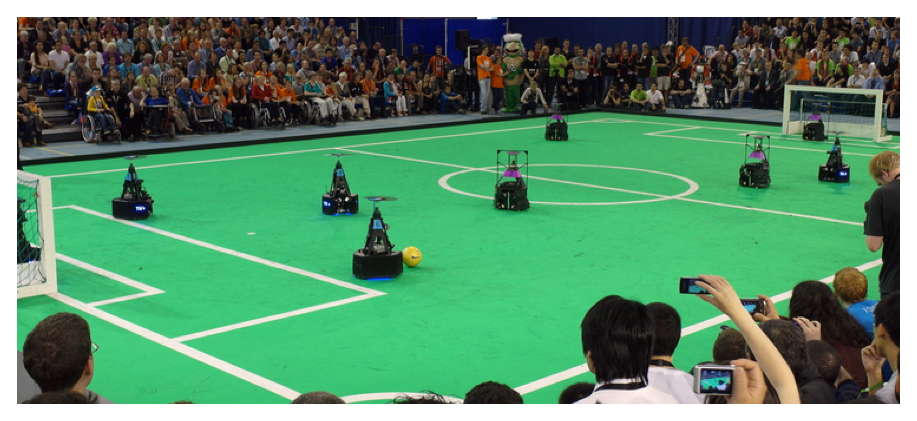
\includegraphics[width=15.0cm]{figure/Observation_target_game_C.eps}
    \caption{Observation target game C}
    \label{fig:C}
    
  \end{center}
\end{figure}

\clearpage%-------------------------図-----------------------------------------


\subsection{状況分析における観察要素の設定}
試合を観察するにあたり,まず,用意に観察可能な要素を対象として設定する.対象としては,選手やボールの座標や速度に加え,試合経過時間や,得失点差なども考えられる.今回は,人間による試合の観察方法として,試合フィールド全体を,単眼カメラを用いて撮影する方法を選択したため,フィールド内での様々な座標データをもとに,単眼カメラを用いて撮影する方法を選択したため,フィールド内での様々な座標データをもとに,状態空間を張る.人間による試合・ロボットによる試合どちらとも,2チームの選手同士5対5で行い,全選手とボールの意志座標をピクセル座標からフィールド座標に変換して取得した.(Fig\ref{fig:Settiong}参照)
また,観察ベクトル$A$を式(\ref{6})で示す.

\begin{equation}
\label{6}
A = [P_{k=1}, P_{k=2}, \cdots, P_{k=10}, B]
\end{equation}

ただし,フィールドでの選手位置座標$P_k$, ボール座標$B$については(\ref{7}),(\ref{8})に示す.ここで,$k$は選手識別のためのIDであり,$k=1,2,3,4,5$の選手で構成されるチーム1と$k = 6,7,8,9,10$の選手で構成されるチーム2での試合を観察ている.なお,$k = 5,10$は両チームのギールキーパーである.

\begin{equation}
\label{7}
P_k = [P_{x_k}, P_{y_k}]
\end{equation}

\begin{equation}
\label{8}
B = [B_{x}, B_{y}]
\end{equation}

\clearpage %-------------------------図-----------------------------------------

\begin{figure}[ht]
  \begin{center}
  
    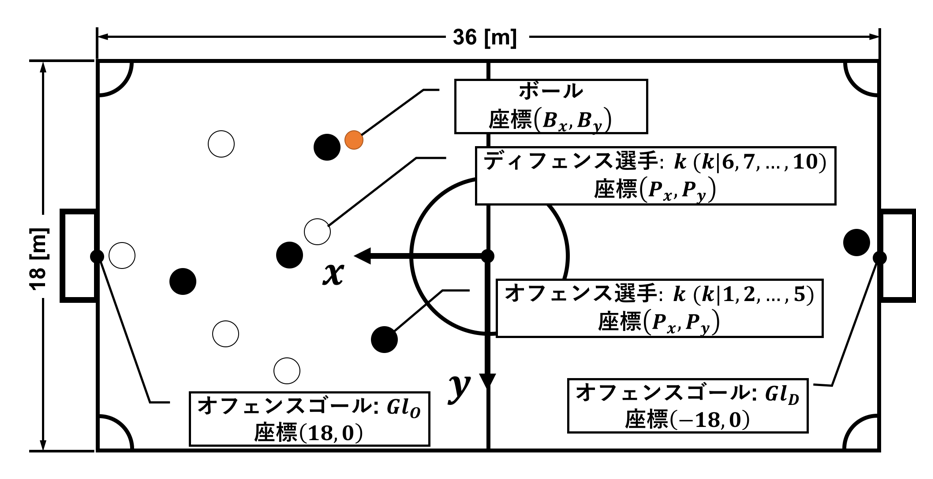
\includegraphics[clip,width=15.0cm]{figure/The_Observation_Environment_of_the_Game.eps}
    \caption{The Observation Environment of the Game}
    \label{fig:Setting}
    
  \end{center}
\end{figure}

\clearpage%-------------------------図-----------------------------------------

\subsection{チーム行動の有無による変化}
\subsubsection{実験方法}
まず,人間同士の試合A,Bを比較して,チーム行動の慣れ具合により違いが生じるかを観測した.入力ベクトルを,式(\ref{9})に示す.

\begin{equation}
\label{9}
v^{\mu} = [P_k, B]
\end{equation}

評価は,近傍ユニットとのユークリッド距離によるクラスタ配置の違いと,Fig\ref{fig:Defining}に示すように,ボールに一番近い選手からアルファベータガンマと割り振った際,学習が収束した後の各入力ベクトルに対する最整合ユニット(BMU)の配置に対して行う.また,クラスタが明確に生成可能かどうかも観察する.

\subsubsection{実験結果}
まず,試合Aについて,各パラメータをTable\ref{table:2}に示す.また,作成したSOMの特徴マップをFig.\ref{fig:SOM_result01},\ref{fig:SOM_result02}に示す.ここで,色のグラデーションは,近傍のユニットとの距離が遠くなるにつれて赤色,近くなるにつれて,青色のグラデーションで示している.つまり,青いユニットの集団は類似している重みベクトルが配置されていることとなる.同様に表\ref{table:3},Fig.\ref{fig:SOM_result03},\ref{fig:SOM_result04}に試合Bについてのパラメータおよび作成したSOMの特徴マップを示す.

\begin{table}[htb]
	\begin{center}
	\caption{SOM parameters for experiment (Observation target game A)}
	\begin{tabular}{|c|c|c|}\hline
		\label{table:2}
	 	パラメータ名 & 変数 & 値  \\ \hline \hline
	 	学習回数 & $T$ & 10  \\
   	 	入力データ数 & $M$ & 300 \\
		マップサイズ & - & 15×15 \\
   		初期近傍半径 & $\sigma_{\Lambda_0}$ & 0.8 \\ \hline
	\end{tabular}
	\end{center}
\end{table}

\begin{table}[t]
	\begin{center}
	\caption{Role sharing by the relative distance between the player and the ball among the players in the team (Observation target game A)}
	\begin{tabular}{|c|c|c|}\hline
		\label{table:3}
	 	パラメータ名 & 変数 & 値  \\ \hline \hline
	 	学習回数 & $T$ & 10  \\
   	 	入力データ数 & $M$ & 400 \\
		マップサイズ & - &20×20\\
   		初期近傍半径 & $\sigma_{\Lambda_0}$ & 0.8 \\ \hline
	\end{tabular}
	\end{center}
\end{table}

\subsubsection{考察}
Fig.\ref{fig:SOM_result01},Fig.\ref{fig:SOM_result02}からわかるように,チームプレーに慣れていない選手群の試合では,ボールに対するチーム内での選手の相対的距離により,クラスタが分けられることはなかった.しかし,Fig.\ref{fig:SOM_result03}, Fig.\ref{fig:SOM_result04}からわかるように,チームプレーに慣れている選手群の試合では,クタスタリングされた.図で赤いユニットによって大きく二つのクラスタに分けられ,そこでボールに近いアルファとベータの群と,遠いデルタ,ガンマの群は大きく分けられた.このことから,チームプレーに慣れている選手から構成されているチームのほうが,チームプレーに慣れていない選手から構成されているチームよりもチーム内での自分のボールへの相対的近さに対する行動選択への影響が大きいことがわかる.

\clearpage %-------------------------図-----------------------------------------

\begin{figure}[htb]
  \begin{center}
    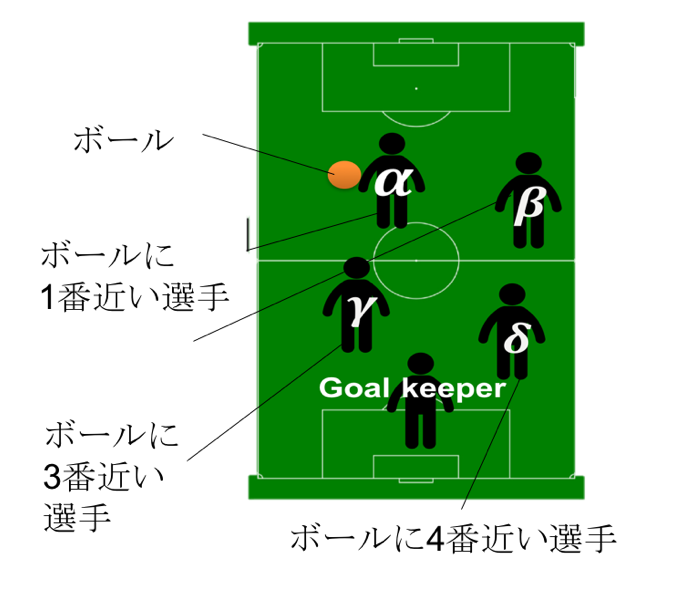
\includegraphics[clip,height=10cm]{figure/Defining_the_position_by_the_relative_distance_within_the_team_relative_to_the_ball.eps}
    \caption{Defining the position by the relative distance within the team relative to the ball}
    \label{fig:Defining}
 \end{center}
\end{figure}

\begin{figure}[htb]
  \begin{center}
      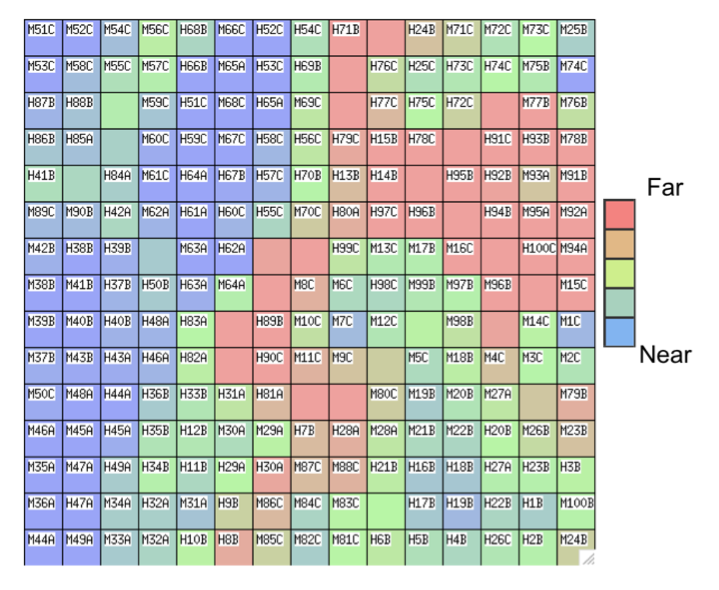
\includegraphics[clip,height=8.0cm]{figure/The_feature_map_expressed_by_the_gradation_display_Observation_target_game_A.eps}
    \caption{The feature map expressed by the gradation display (Observation target game A)}
    \label{fig:SOM_result01}
\end{center}
\end{figure}

\begin{figure}[htb]
  \begin{center}
    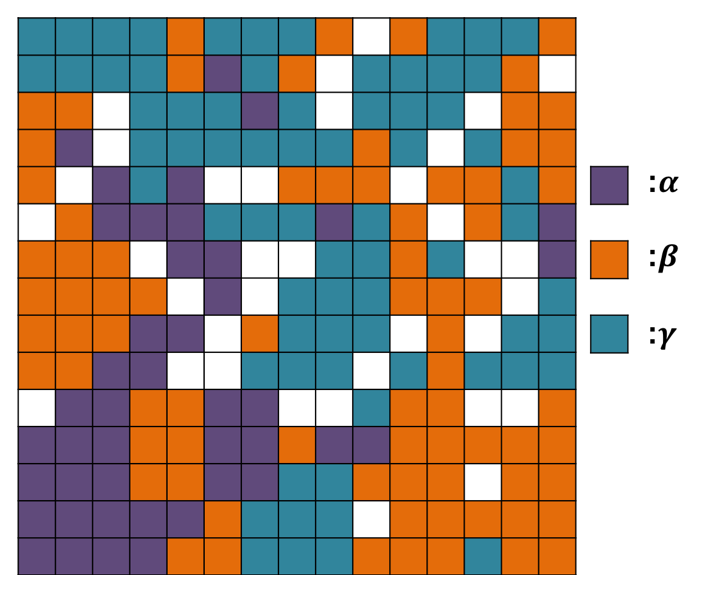
\includegraphics[clip,height=8.0cm]{figure/Role_sharing_by_the_relative_distance_between_the_player_and_the_ball_among_the_players_in_the_team_Observation_target_game_A.eps}
    \caption{Role sharing by the relative distance between the player and the ball among the players in the team (Observation target game A)}
    \label{fig:SOM_result02}
  \end{center}
\end{figure}

\begin{figure}[htb]
  \begin{center}
    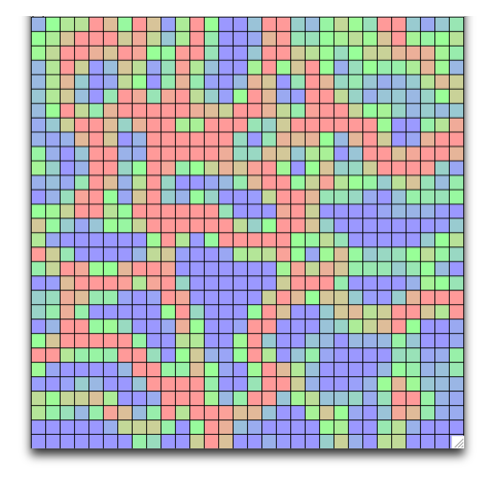
\includegraphics[clip,height=8.0cm]{figure/The_feature_map_expressed_by_the_gradation_display_Observation_target_game_B.eps}
    \caption{The feature map expressed by the gradation display (Observation target game B).eps}
    \label{fig:SOM_result03}
  \end{center}
\end{figure}

\begin{figure}[htb]
  \begin{center}
    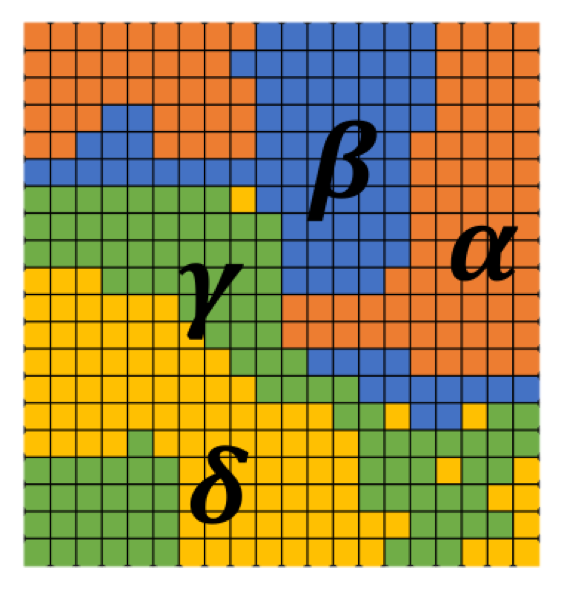
\includegraphics[clip,height=8.0cm]{figure/Role_sharing_by_the_relative_distance_between_the_player_and_the_ball_among_the_players_in_the_team_Observation_target_game_B.eps}
    \caption{Role sharing by the relative distance between the player and the ball among the players in the team (Observation target game B)}
    \label{fig:SOM_result04}
  \end{center}
\end{figure}

\clearpage%-------------------------図-----------------------------------------


\subsection{チーム内での仲間との位置関係}

\subsubsection{実験方法}
次に,人間同士の試合Bについて,チーム内での仲間の選手の行動を入力ベクトルに入れ,仲間との位置関係により,クラスタリングが可能かどうかを観察する.入力ベクトルを,式(\ref{10})に示す.

\begin{equation}
	\label{10}
	v^{\mu} = [P_k, P_2, P_3, P_4, B]
\end{equation}

評価は,近傍ユニットとのユークリッド距離によるクラスタリングと,ゴールキーパー以外の仲間の選手からできる四角形の面積の大きさを見ることで,選手の疎密具合による最整合ユニット(BMU)の最近ユニットとのユークリッド距離によるクラスタと一致しているかを確かめる.仲間の選手4人の位置座標と頂点とする四角形の面積を用いた評価関数は三斜法に基づき式(\ref{11})により導出した.ここでdは,1チームの4人の選手をx座標値が小さい順に並べ直した時の各位置座標のIDである.

\begin{equation}
	\label{11}
	Y = \frac{1}{2}\Sigma(P_{x_d}-P_{x_{d+1}})(P_{y_d}+P_{y_{d+1}})
\end{equation}

各パラメータをTable\ref{table4}に示す.また,作成したSOMの特徴マップをFig.\ref{fig:SOM_result05}-\ref{fig:SOM_result08}に示す.

\begin{table}[t]
	\begin{center}
	\caption{Role sharing by the relative distance between the player and the ball among the players in the team (Observation target game A)}
	\begin{tabular}{|c|c|c|}\hline
		\label{table4}
	 	パラメータ名 & 変数 & 値  \\ \hline \hline
	 	学習回数 & $T$ & 10  \\
   	 	入力データ数 & $M$ & 400 \\
		マップサイズ & - &20×20\\
   		初期近傍半径 & $\sigma_{\Lambda_0}$ & 0.8 \\ \hline
	\end{tabular}
	\end{center}
\end{table}

\subsubsection{考察}
まず,Fig ??を見ると,大きく4つのクラスタが観測できる.右上から左下にかけての協会と左右を分けるように上下に伸びる境界が見て取れる.
しかし,Fig??, Fig??, Fig??を観察すると,どれもこのクラスタと合致するようにクラスタ生成がなされていない.次にFig??, Fig??を観察すると,オフェンス,ディフェンス両方のチームで特徴マップ上部の色が赤と青とで対象的である.この部分は,Fig ??からボールがオフェンスチームが攻めるゴールから遠い時を示している.したがって,オフェンスチームは自陣の攻めるゴールからボールが遠くなると密集し,対象雨滴にディフェンスチームは自陣が守るゴールからボールが遠くなると分散したポジショニングをしていることがわかる.

\clearpage %-------------------------図-----------------------------------------

\begin{figure}[htb]
  \begin{center}
      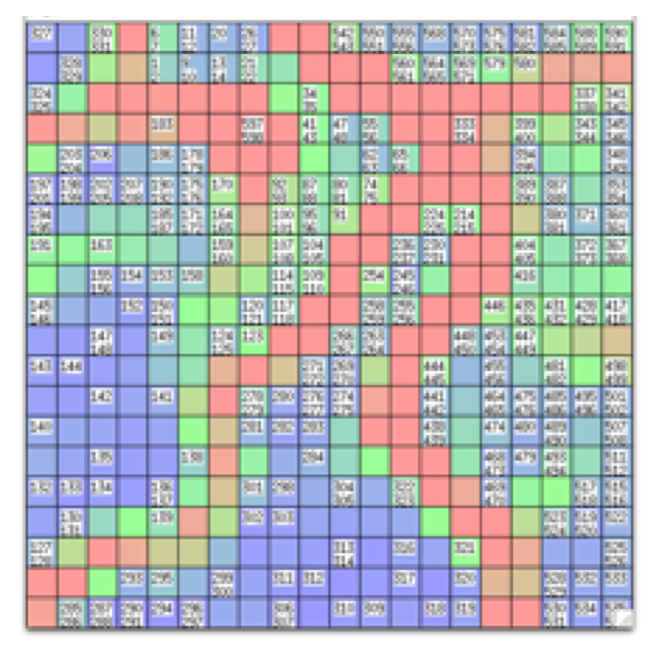
\includegraphics[clip,height=5.5cm]{figure/The_feature_map_expressed_by_the_gradation_display_Observation_target_game_B_2.eps}
    \caption{The feature map expressed by the gradation display (Observation target game B)}
    \label{fig:SOM_result05}
\end{center}
\end{figure}

\begin{figure}[htb]
  \begin{center}
    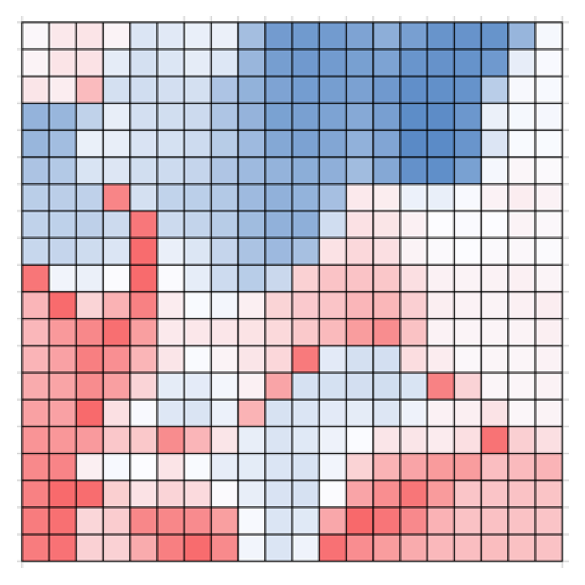
\includegraphics[clip,height=5.5cm]{figure/The_area_of_the_rectangle_constituted_with_the_player_of_the_defense_team_as_the_apex_Observation_target_game_B.eps}
\caption{The area of the rectangle constituted with the player of the defense team 
as the apex (Observation target game B)}
    \label{fig:SOM_result06}
  \end{center}
\end{figure}

\begin{figure}[htb]
  \begin{center}
    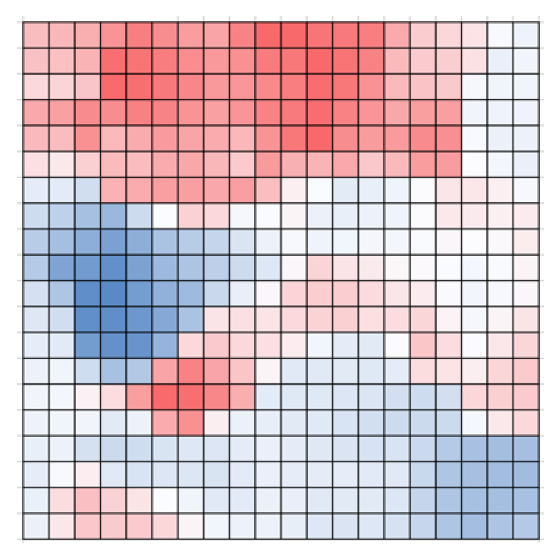
\includegraphics[clip,height=8.0cm]{figure/The_area_of_the_rectangle_constituted_with_the_player_of_the_offense_team_as_the_apex_Observation_target_game_B.eps}
    \caption{The area of the rectangle constituted with the player of the offense team
 as the apex (Observation target game B)}
    \label{fig:SOM_result07}
  \end{center}
\end{figure}

\begin{figure}[htb]
  \begin{center}
    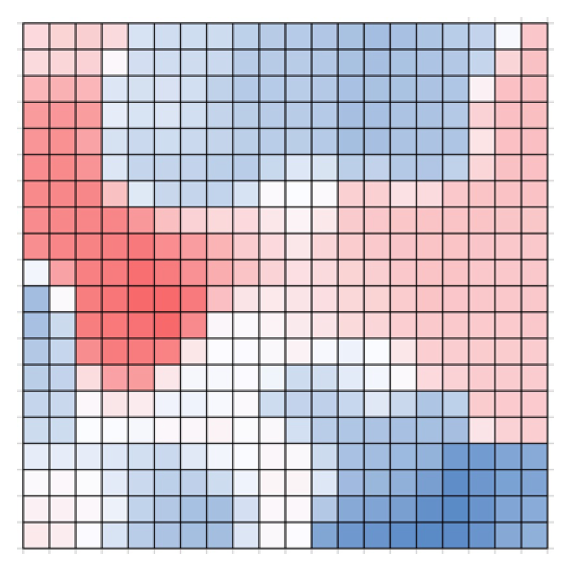
\includegraphics[clip,height=8.0cm]{figure/Distance_of_the_ball_against_the_goal_attacked_by_the_offense_team_Observation_target_game_B.eps}
    \caption{Distance of the ball against the goal attacked by the offense team(Observation target game B)}
    \label{fig:SOM_result08}
  \end{center}
\end{figure}

\clearpage%-------------------------図-----------------------------------------


\subsection{人間同士によるフットサル試合とロボット同士によるサッカー試合の比較解析}
全選手が参加している状態において,セットプレイからシュートまでの選手・ボール位置座標を用いたSOMによるクラスタリングを行い,試合状況の解析を行う.ここにおいて,セットプレイとは,キックオフ・フリーキック・コーナーキックなど,試開始に際しボールをセットして行うプレーを指す. SOMの学習において,入力ベクトル9次元であり,次式(\ref{12})で示す.

\begin{equation}
	\label{12}
	v^{\mu} = [P_k, P_2, P_3, P_4, P_6, P_7, P_8, P_9, B]
\end{equation}
ここで,今回はゴールキーパー以外を対象とするため,ゴールキーパーである k=5,10 以外の  k=1,2,3,4 および$k=6,7,8,9$ 選手位置座標を用いる.以降簡単のために,k=1,2,3,4の選手で構成されるチームを赤チーム.$k=6,7,8,9$の選手で構成されるチームを青チームとする.また,以下の選定条件によりデータを取捨選択した.
\begin{enumerate}
  \item セットプレイからシュートまでの一連のプレ-であること
  \item 1トライで選手の交代が行われていないこと
\end{enumerate}
 ここで1トライとは,1回のセットプレイからシュートまでのことである.今回入力データとして用いたトライは以下Fig.??の計10トライである.
 
 \subsubsection{学習パラメータ}
 Table\ref{table5}に本実験においての,SOMのパラメータを示す.
 
\begin{table}[htb]
	\begin{center}
	\caption{SOM parameters for experiment(Observation target game B,C)}
	\begin{tabular}{|c|c|c|}\hline
		\label{table5}
	 	パラメータ名 & 変数 & 値  \\ \hline \hline
	 	学習回数 & $T$ & 10  \\
   	 	入力データ数 & $M$ & 200 \\
		マップサイズ & - &30×30\\
   		初期近傍半径 & $\sigma_{\Lambda_0}$ & 0.8 \\ \hline
	\end{tabular}
	\end{center}
\end{table}

\subsubsection{実験結果}
実験の結果1つの特徴マップを作成した.ユークリッド距離による色のグラデーションをFig??に示す.赤い部分がユークリッド距離の大きい部分となる.\\
 また,クラスタリングされた学習終了後の特徴マップに,各入力ベクトルの最終的な最整合ニューロン(BMU)を付加したものをFig ??に示す.黒く示した部分が,ユークリッド距離が大きいニューロンであり,赤や青で示した部分が,赤チームや青チームが最終的にシュートに漕ぎ着けたトライの入力ベクトルが選択した最整合ニューロンである.

\subsubsection{考察}
攻めるチームが,赤チームか青チームという違いで大きく選択したクラスが異なった.これは,攻めるときと守るときで,チーム内でのフォーメーションが大きく異なることを示している.この時は,セットプレーからシュートまでを1トライと換算し,入力した.人間の試合では結果,赤チームがセットプレーからシュートまでボールを奪われずにゴールした時,青チームがセットプレーからシュートまでボールを奪われずにゴールした時,赤チームがセットプレーを始めたが途中で青チームに奪われてしまった時,青チームがセットプレーを始めたが途中で赤チームに奪われてしまった時のすべての場合が,違うクラスタに分類された.

\clearpage

\begin{figure}[ht]%------------------------------図--------------------------------------
  \begin{center}
  
    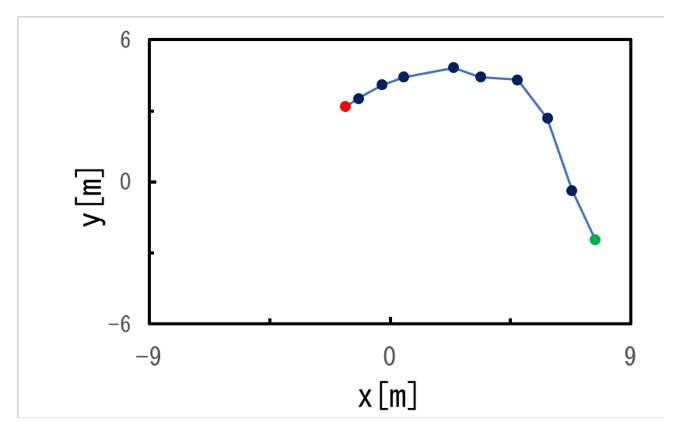
\includegraphics[clip,width=15.0cm]{figure/TRY01_red_to_red.eps}
    \caption{TRY01 red to red}
    \label{fig:try01}
    
    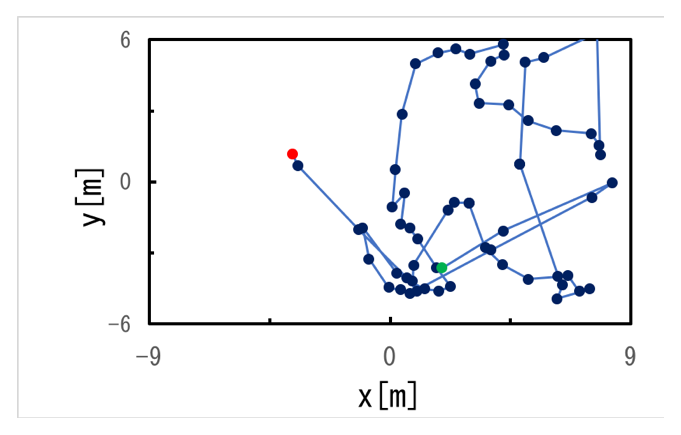
\includegraphics[width=15.0cm]{figure/TRY02_red_to_red.eps}
    \caption{TRY02 red to red}
    \label{ig:try02}
    
  \end{center}
\end{figure}

\begin{figure}[ht]
  \begin{center}

    
    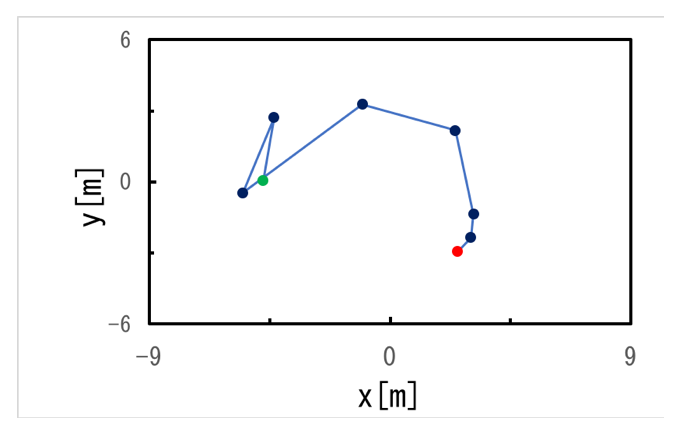
\includegraphics[clip,width=15.0cm]{figure/TRY03_blue_to_blue.eps}
    \caption{TRY03 blue to blue}
    \label{fig:try03}
    
    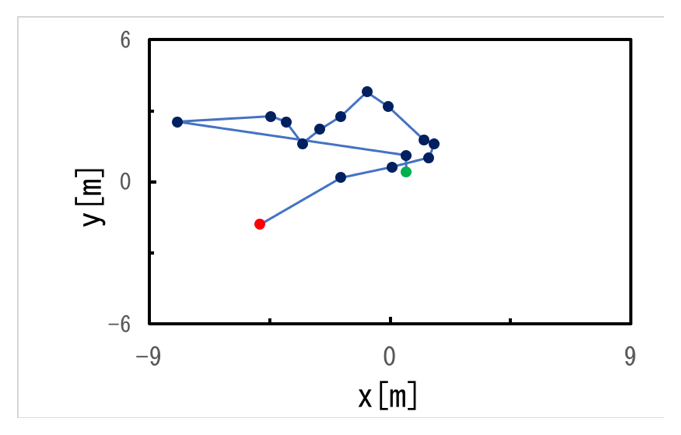
\includegraphics[width=15.0cm]{figure/TRY04_red_to_blue.eps}
    \caption{TRY04 red to blue}
    \label{ig:try04}

  \end{center}
\end{figure}

\begin{figure}[ht]
  \begin{center}
    
    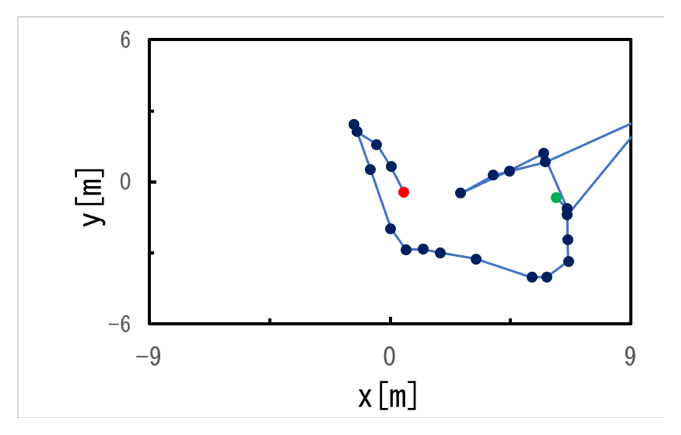
\includegraphics[clip,width=15.0cm]{figure/TRY05_red_to_red.eps}
    \caption{TRY05 red to red}
    \label{fig:try05}
    
    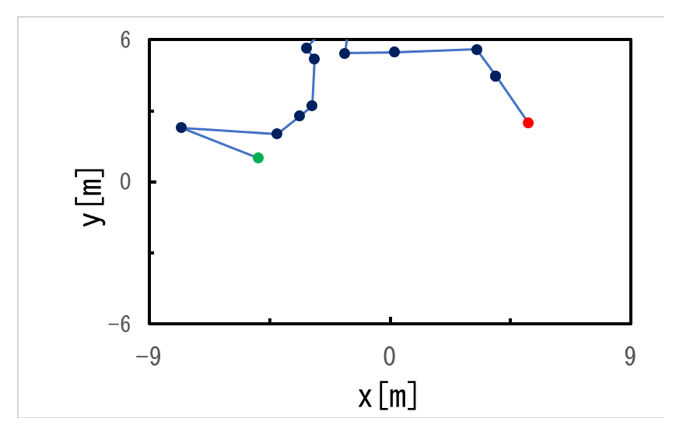
\includegraphics[width=15.0cm]{figure/TRY06_blue_to_blue.eps}
    \caption{TRY06 blue to blue}
    \label{ig:try06}
    
  \end{center}
\end{figure}

\begin{figure}[ht]
  \begin{center}
    
    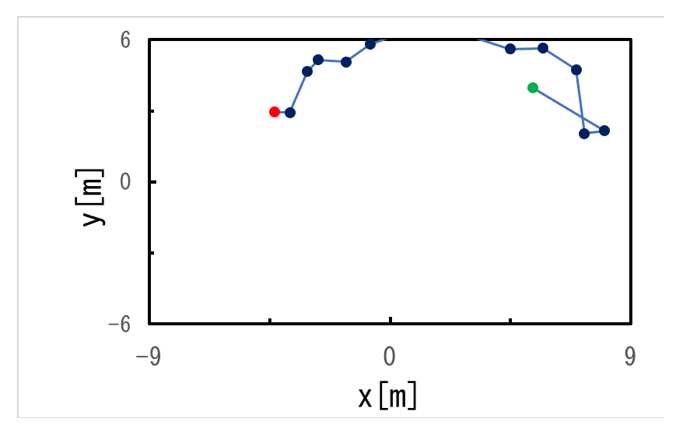
\includegraphics[clip,width=15.0cm]{figure/TRY07_red_to_red.eps}
    \caption{TRY07 red to red}
    \label{fig:try07}
    
    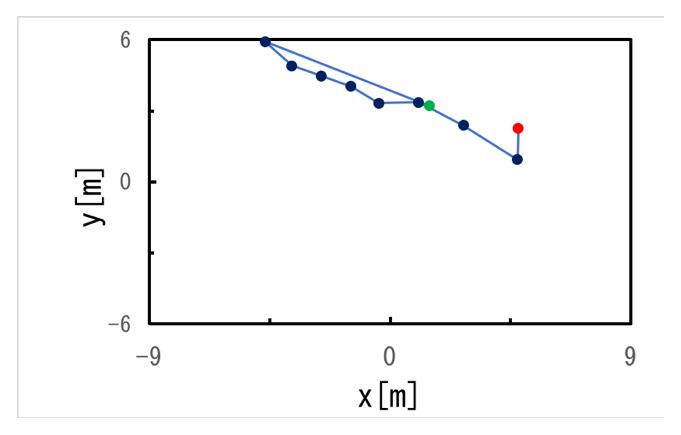
\includegraphics[width=15.0cm]{figure/TRY08_blue_to_blue.eps}
    \caption{TRY08 blue to blue}
    \label{ig:try08}
    
  \end{center}
\end{figure}

\begin{figure}[ht]
  \begin{center}
    
    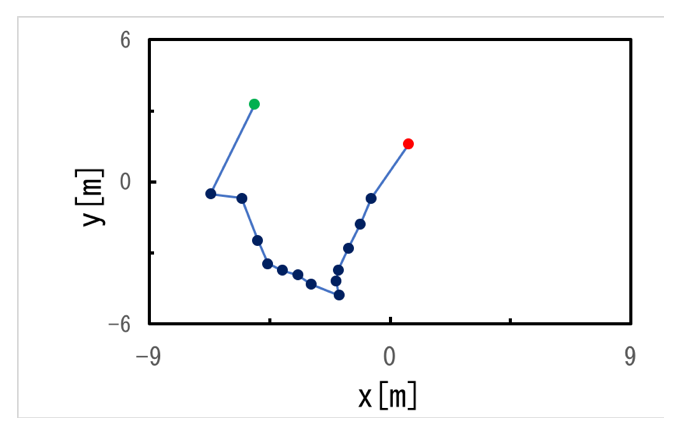
\includegraphics[clip,width=15.0cm]{figure/TRY09_blue_to_blue.eps}
    \caption{TRY09 blue to blue}
    \label{fig:try09}
    
    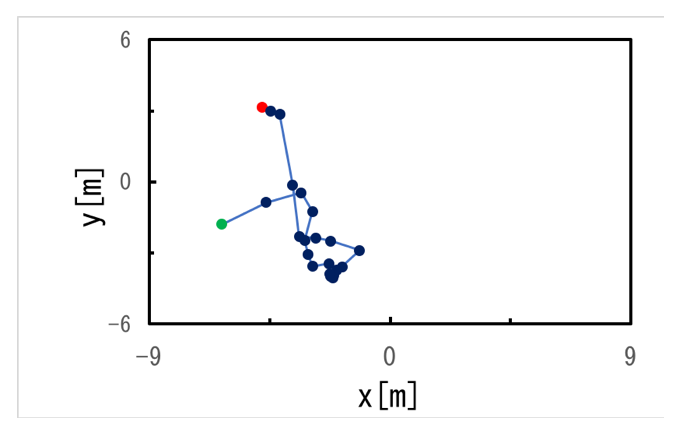
\includegraphics[width=15.0cm]{figure/TRY10_red_to_blue.eps}
    \caption{TRY08 red to blue}
    \label{ig:try010}
    
  \end{center}
\end{figure}

\begin{figure}[ht]
  \begin{center}
  
    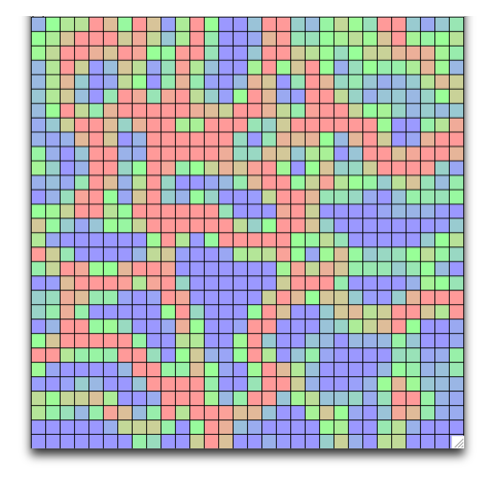
\includegraphics[clip,width=10.0cm]{figure/The_feature_map_expressed_by_the_gradation_display_Observation_target_game_B.eps}
    \caption{The feature map expressed by the gradation display
(Observation target game B)}
    \label{fig:SOM_result09}
    
    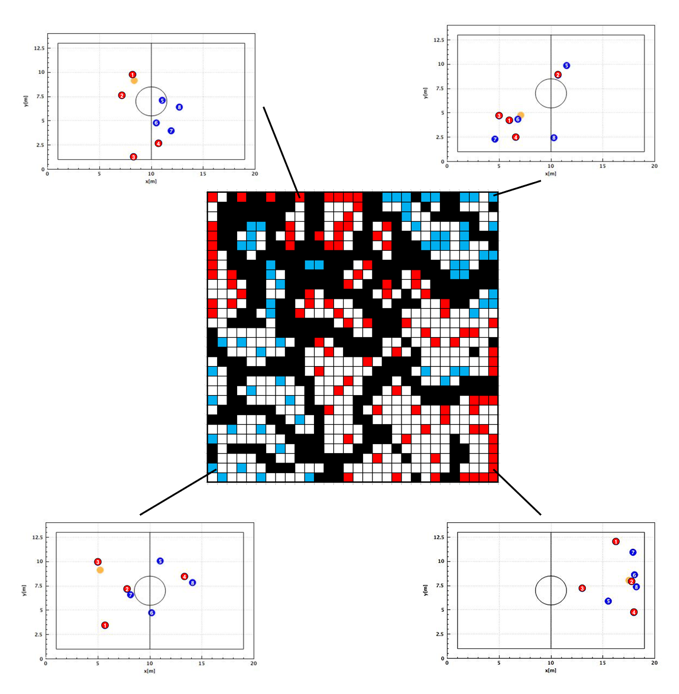
\includegraphics[width=10.0cm]{figure/A_color-coded_figure_with_the_team_try_finally_chosen_shot_Black_Euclidean_distance_more_than_0.6.eps}
    \caption{A color-coded figure with the team try finally chosen a shot(Black : Euclidean distance $\geq$ 0.6)}
    \label{fig:SOM_result10}
    
  \end{center}
\end{figure}

\begin{figure}[ht]
  \begin{center}
  
    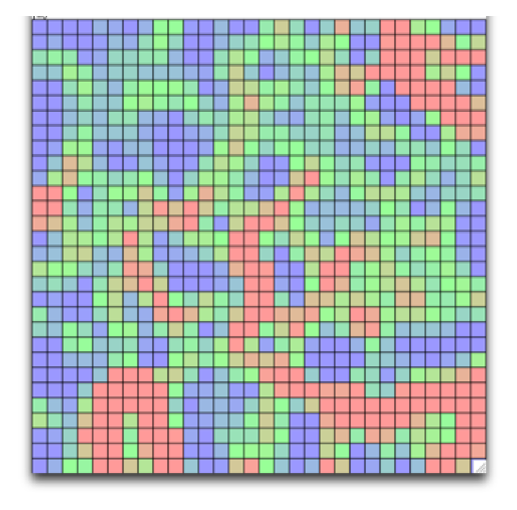
\includegraphics[clip,width=10.0cm]{figure/The_feature_map_expressed_by_the_gradation_display_Observation_target_game_C.eps}
    \caption{The feature map expressed by the gradation display 
(Observation target game C)}
    \label{fig:SOM_result11}
    
    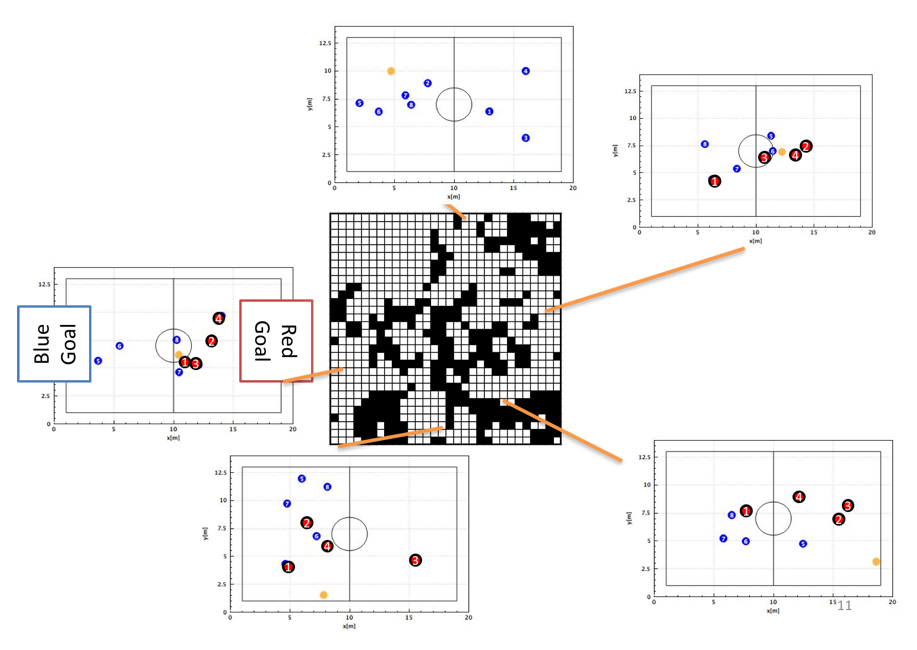
\includegraphics[width=10.0cm]{figure/A_color-coded_figure_with_the_team_try_Black_Euclidean_distance_0.6.eps}
    \caption{A color-coded figure with the team try 
(Black : Euclidean distance $\geq$ 0.6)}
    \label{fig:SOM_result12}
    
  \end{center}
\end{figure}



\clearpage%------------------------------図--------------------------------------


\subsection{結論}
本章では,人とロボットの協調にむけたマルチエージェントゲームの行動快解析を目標として,3つの実験を行なった.全て,人間同士の試合もしくはロボット同士の試合を観察することで,位置座標から得られる試合情報がどのくらいクラスタリング要素として有効かということを調べた.\\
 まず,1つ目の実験では,各選手とボールの4次元での入力であったが,普段からチームとして行動に慣れている選手群と,慣れていない選手群では,大きく異なった.慣れている選手群には,SOMの特徴マップからユークリッド距離によりクラスタリングされた結果から見て取れる境界で,チーム内での選手のボールへの近さも分かれていた.これは,慣れていないチームでの試合との比較をすることにより,より明確化される.人間の試合でも,即席では「チームで協調」することができない場面があることを示している.\\
 次に,同チームの選手群でできる四角形の面積を求めることにより,チーム内での選手の疎密度を観察した.すると,試合中において攻める局面と守る局面では,疎密度が真逆になることがわかった.ここまでの,実験で,仲間の情報を含んだ場合の選手の行動選択を観察することができた.\\
 最後に,相手選手も含めたSOMの特徴マップを作成することにより,試合全体の観察を行なった.この時は,セットプレーからシュートまでを1トライと換算し,入力した.人間の試合では結果,赤チームがセットプレーからシュートまでボールを奪われずにゴールした時,青チームがセットプレーからシュートまでボールを奪われずにゴールした時,赤チームがセットプレーを始めたが途中で青チームに奪われてしまった時,青チームがセットプレーを始めたが途中で赤チームに奪われてしまった時のすべての場合が,違うクラスタに分類された.これは,ユークリッド距離によるクラスタ配置とも一致しており,セットプレーからシュートまでの1トライが大きなクラスタの一つの中で動いており,試合状況のクラスタリングが可能であることを示している.\\
  一方,ロボットの試合では,人間同様に解析を行ったが,まったくクラスタリングできなかった.このことから,ロボカップ中型リーグでは,ロボットの協調が人間の協調と大きく異なっていることを示している.\\
 今後の展望として,このように,クラスタリングできたSOMをロボットに導入することで,現在の試合状況の理解をロボットにされることを考える.




 





















